% !TEX program = xelatex
\documentclass[11pt,a4paper]{article}
\usepackage[margin=2.1cm]{geometry}
\usepackage{fontspec}
\newfontfamily\jp{Hiragino Kaku Gothic Pro}
\usepackage{microtype}
\usepackage{booktabs}
\usepackage{tabularx}
\usepackage{array}
\usepackage{xcolor}
\usepackage{enumitem}
\usepackage{caption}
\usepackage{float}
\usepackage{tikz}
\usetikzlibrary{arrows.meta,positioning,shapes.geometric,calc,fit,backgrounds}
\usepackage{pgfplots}
\pgfplotsset{compat=1.18}
\usepgfplotslibrary{groupplots}
\usepackage[hidelinks]{hyperref}

% ---------- palette ----------
\definecolor{cTop}{HTML}{2B6CB0}
\definecolor{cMid}{HTML}{9F7AEA}
\definecolor{cLow}{HTML}{A0AEC0}
\definecolor{cOurs}{HTML}{D9480F}
\definecolor{cOpp}{HTML}{2F855A}
\definecolor{cGood}{HTML}{2F855A}
\definecolor{cBad}{HTML}{C53030}
\definecolor{cInk}{HTML}{2D3748}
\definecolor{cSoft}{HTML}{EDF2F7}

% ---------- source / code macros ----------
\newcommand{\scratch}{file:///private/tmp/claude-501/-Users-tristanbasri-Desktop-Code-cambridge-battlecode-s2/b3f4cb6b-e46a-405f-957c-42c44c05c8dc/scratchpad/ladder-data}
\newcommand{\repo}{file:///Users/tristanbasri/Desktop/Code/cambridge-battlecode-s2}
% \src{url}{label}: inline source citation
\newcommand{\src}[2]{{\small(\href{#1}{\textcolor{cTop}{\texttt{#2}}})}}
% \code{repo-relative-path}{display}: clickable code reference to our bot
\newcommand{\code}[2]{\href{\repo/#1}{\texttt{\textcolor{cOurs!80!black}{#2}}}}
\newcommand{\vfive}{bots/bot-v5-r175199/src}
\newcommand{\CI}{C\&I}
\newcommand{\viz}{file:///private/tmp/claude-501/-Users-tristanbasri-Desktop-Code-cambridge-battlecode-s2/b3f4cb6b-e46a-405f-957c-42c44c05c8dc/scratchpad/viz2}

\setlength{\parskip}{0.45em}
\setlength{\emergencystretch}{2em}
\setlength{\parindent}{0pt}
\captionsetup{font=small,labelfont=bf}

\title{\vspace{-1.2cm}\textbf{Top teams win the gold race early}\\[0.3em]
\large Strategies, techniques and faults on the Cambridge Battlecode 2026a ladder, and where our bot falls short}
\author{Research report on ladder data from 2026-10-21 and 2026-10-22}
\date{22 October 2026}

\begin{document}
\maketitle

\noindent\colorbox{cSoft}{\parbox{\dimexpr\linewidth-2\fboxsep}{\small
\textbf{Bottom line.} The top 20 teams on the 2026a ladder share no secret technique. They win the \textbf{economy race between rounds 100 and 500} and they almost never waste turns. A team that leads on gold earned at round 300 wins \textbf{73.9\%} of games, and a lead of 400 gold or more wins \textbf{86\%}. Top-20 teams have about \textbf{300 more gold than ranks 51--150 by round 300}, and they \textbf{die half as often} (7.2 against 15.2 deaths per game). Since the balance patch they have all moved to one core (Heart of Ruin, Vesper Vale, Marcella, Vendetta, Ryth), drafted as a fixed function of the map. Each team then runs one clear win plan on top of that core: a stat-stacked carry, a Prism gem bank, or pure farming. Our team, \emph{Anime girls against \#2 period cramp} (about \#97--\#108, rating about 1750--1765), is a strong fighting bot. In wins it gets 23 kills to 6, and it beats weaker teams 24--1. Against peers that avoid fights it loses: it is \textbf{9--16 against teams within about 10 ladder places}, and it is already behind on gold at round 300 in those losses (982 against 1,199). The largest fault we found is self-inflicted. \textbf{About 8.6\% of our champion turns run out of fuel}, against 0.5\% for our opponents and about zero for ranks 1--3, and almost all of it comes from the farm planner. A gem-carry draft (Marcella then Prism) that went live on weak evidence is \textbf{2--6} on the maps where it fires. The fixes are in order: stop the fuel spills, retire or gate the gem-carry draft, and close the round-100-to-500 gold gap. Map-specific bugs on 01boss\_battle and 01islands come next. \textbf{Decoded replays} (Section~\ref{sec:replays}) add the movement picture: top teams \textbf{invade} (21\% of their time in the enemy half against top-20 opponents' 11\%) and \textbf{stay together}, while our bot \textbf{stands still on 45\% of its alive rounds}, more than any top-20 team.}}

\vspace{0.6em}
{\small\textbf{Data windows.} The \emph{ladder-wide statistics} come from part 1 of 19 of the organiser's 2026-10-21 dump: 23,401 summaries on engines 1.0.1/1.0.2, with buckets set by the 2026-10-22 ladder ranks \src{\scratch/matchdb/out/}{matchdb/out}. The \emph{top-20 team analyses} and \emph{our own 50 ranked games} all come from 2026-10-22 (about 16:20--19:30 UTC, engine 1.0.3), so they reflect current submissions \src{\scratch/top1-10/agg_current.txt}{top1-10/agg\_current.txt}, \src{\scratch/top11-20/agg_recent.txt}{top11-20/agg\_recent.txt}, \src{\scratch/ours/rows.json}{ours/rows.json}. Drafts changed sharply between the two days, so every draft finding is quoted from the 10-22 data. Earlier notes listed ``Sydney's Realist'' (SR) and ``Latent Tactics'' (LT) as candidates for our team. They are not us. Both are comparison teams in our rating band, and Latent Tactics beat us 3--2. Our team appears as ``AG'' in the dump, with only 13 ranked games. The \emph{replay analysis} (Section~\ref{sec:replays}) decodes 1,745 full replays from part 1 of the 10-21 replay dump, so it describes the \emph{previous day's} submissions; one 10-22 replay of ours is used where marked \src{\viz/an/features.jsonl}{viz2/an/features.jsonl}.}

\tableofcontents

%=====================================================================
\section{Gold earned by round 300 predicts most results}
%=====================================================================

The ladder rewards economic tempo more than anything else. Across 23,373 decided games in the 10-21 dump, the team with more lifetime gold earned at round 100 wins \textbf{64.9\%} of the time. That rises to \textbf{73.9\% at round 300} and \textbf{78.1\% at round 500} \src{\scratch/matchdb/out/separators.csv}{separators.csv}. Tributed gems overtake gold as the best predictor only after round 750, and by round 1,000 the gem leader wins 86.4\%. That is mostly because the gem leader is about to hit the 1,000-gem win condition. Kill leads are a weaker signal (73.3\% at round 500), and having fewer deaths is weaker still (68.6\%). Figure~\ref{fig:sep} shows that kills plateau while gold and gems keep rising. Kills matter mostly because they move gold and steal carried gems.

\begin{figure}[H]
\centering
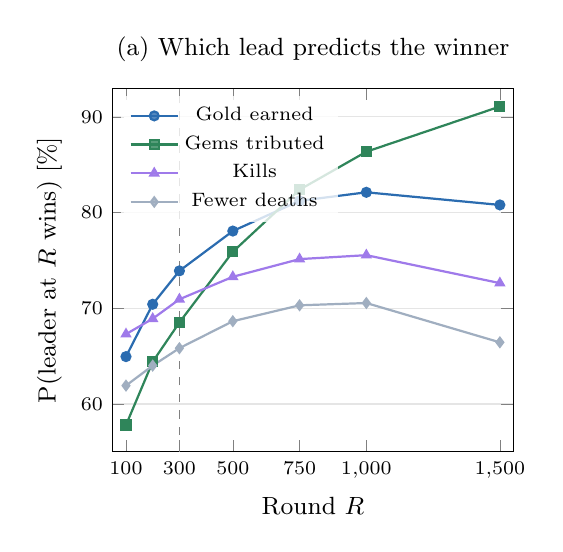
\begin{tikzpicture}
\begin{axis}[
  width=0.55\linewidth, height=6.2cm,
  xlabel={Round $R$}, ylabel={P(leader at $R$ wins) [\%]},
  xmin=50, xmax=1550, ymin=55, ymax=93,
  xtick={100,300,500,750,1000,1500},
  ymajorgrids, grid style={gray!20},
  legend style={font=\scriptsize, at={(0.02,0.98)}, anchor=north west, draw=none, fill=white, fill opacity=0.8, text opacity=1},
  tick label style={font=\scriptsize}, label style={font=\small},
  every axis plot/.append style={thick, mark size=1.6pt},
  title={\small (a) Which lead predicts the winner}
]
\addplot[cTop, mark=*] coordinates {(100,64.95)(200,70.42)(300,73.91)(500,78.07)(750,81.23)(1000,82.12)(1500,80.80)};
\addlegendentry{Gold earned}
\addplot[cOpp, mark=square*] coordinates {(100,57.80)(200,64.41)(300,68.52)(500,75.90)(750,82.39)(1000,86.36)(1500,91.08)};
\addlegendentry{Gems tributed}
\addplot[cMid, mark=triangle*] coordinates {(100,67.30)(200,68.91)(300,70.94)(500,73.29)(750,75.14)(1000,75.55)(1500,72.63)};
\addlegendentry{Kills}
\addplot[cLow, mark=diamond*] coordinates {(100,61.92)(200,64.01)(300,65.83)(500,68.65)(750,70.31)(1000,70.55)(1500,66.44)};
\addlegendentry{Fewer deaths}
\draw[dashed, gray] (axis cs:300,55) -- (axis cs:300,93);
\end{axis}
\end{tikzpicture}\hfill
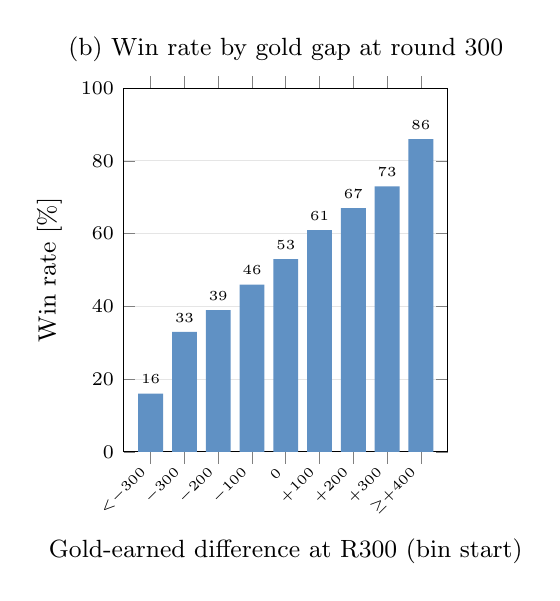
\begin{tikzpicture}
\begin{axis}[
  width=0.47\linewidth, height=6.2cm,
  ybar, bar width=9pt,
  ymin=0, ymax=100, ylabel={Win rate [\%]},
  symbolic x coords={a,b,c,d,e,f,g,h,i},
  xtick=data,
  xticklabels={${<}{-}300$,$-300$,$-200$,$-100$,$0$,$+100$,$+200$,$+300$,${\geq}{+}400$},
  xticklabel style={font=\tiny, rotate=45, anchor=east},
  xlabel={Gold-earned difference at R300 (bin start)},
  ymajorgrids, grid style={gray!20},
  nodes near coords, nodes near coords style={font=\tiny},
  tick label style={font=\scriptsize}, label style={font=\small},
  title={\small (b) Win rate by gold gap at round 300}
]
\addplot[fill=cTop!75, draw=none] coordinates {(a,16)(b,33)(c,39)(d,46)(e,53)(f,61)(g,67)(h,73)(i,86)};
\end{axis}
\end{tikzpicture}
\caption{Ladder-wide separators, 10-21 dump (all CIs $\pm$1pp or less). In (b) the extreme bins hold most games: $n=13{,}289$ below $-300$ and $n=10{,}993$ at $+400$ or more. A gap of 300 gold at round 300 is already decisive five times out of six. Sources: \href{\scratch/matchdb/out/separators.csv}{\texttt{separators.csv}}; gold-difference bins from the per-match feature rows.}
\label{fig:sep}
\end{figure}

This frame matters for everything below. Gold earned early is the variable that best separates top teams from the mid-ladder. It is also where our losses go wrong. These are correlations, since the better bot usually leads on everything. Still, they tell us where to look. A 300-gold deficit at round 300 is recovered fewer than one time in six, so any fault that slows the first 300--500 rounds costs far more than the same fault later. The rules confirm what kills are worth: 100 gold per kill plus any gems the victim carries \src{\repo/docs/GameRules.md}{docs/GameRules.md}.

%=====================================================================
\section{The top 20 converged on one five-champion core after the patch}
%=====================================================================

\subsection{Heart of Ruin, Marcella, Vesper and Vendetta beat the mid-ladder favourites}

The 10-21 dump shows a clean split between what top teams pick and what the rest of the ladder picks (Figure~\ref{fig:picks}a). Heart of Ruin is in \textbf{85.4\%} of top-20 rosters but only 10.3\% of rosters ranked 301 and below. Stellar, Varg and Cassi \& Issac go the other way. The top-20 pick shares are 44.0\%, 19.1\% and 22.7\%; in the 151--300 bucket Stellar is at 69.3\%, and below rank 300 Varg is at 67.8\% and \CI{} at 61.1\% \src{\scratch/matchdb/out/champ_stats.csv}{champ\_stats.csv}. Raw win rates would overstate this, because good teams win with anything. The \emph{team-demeaned} effect compares a champion with the same team's games without it, and it confirms the pattern (Figure~\ref{fig:picks}b). Within the top 20, Heart of Ruin adds \textbf{+9.1pp}, Marcella +6.5pp, Vendetta +5.6pp and Vesper Vale +5.6pp. Stellar costs \textbf{$-$7.3pp} and Prism $-$6.8pp \src{\scratch/matchdb/out/champ_team_demeaned.csv}{champ\_team\_demeaned.csv}. The best pairs are built from the same champions: Marcella + Vesper +2.3pp, Heart of Ruin + Marcella +2.2pp, Vendetta + Vesper +2.6pp. The worst pairs pair Heart of Ruin or Prism with a trap pick (Prism + Vendetta $-$2.9pp; Heart of Ruin + Stellar $-$2.5pp) \src{\scratch/matchdb/out/pair_stats.csv}{pair\_stats.csv}.

\begin{figure}[H]
\centering
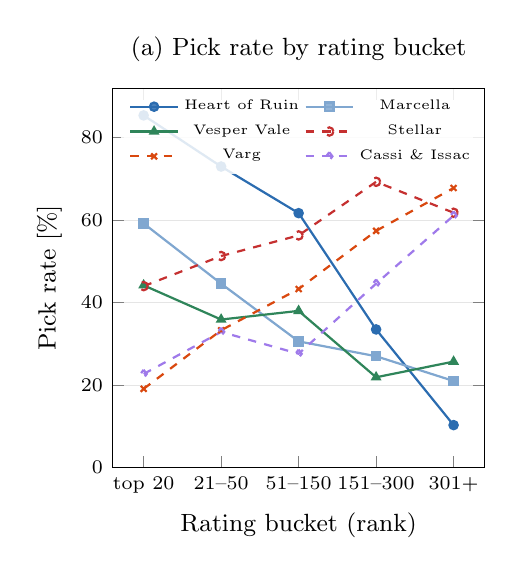
\begin{tikzpicture}
\begin{axis}[
  width=0.52\linewidth, height=6.4cm,
  symbolic x coords={t20,b21,b51,b151,b301},
  xtick=data, xticklabels={top 20,21--50,51--150,151--300,301+}, ymin=0, ymax=92,
  ylabel={Pick rate [\%]}, xlabel={Rating bucket (rank)},
  ymajorgrids, grid style={gray!20},
  tick label style={font=\scriptsize}, label style={font=\small},
  legend style={font=\tiny, at={(1.0,1.0)}, anchor=north east, draw=none, fill=white, fill opacity=0.85, text opacity=1, legend columns=2},
  every axis plot/.append style={thick, mark size=1.5pt},
  title={\small (a) Pick rate by rating bucket}
]
\addplot[cTop, mark=*] coordinates {(t20,85.4)(b21,73.0)(b51,61.7)(b151,33.5)(b301,10.3)}; \addlegendentry{Heart of Ruin}
\addplot[cTop!60, mark=square*] coordinates {(t20,59.2)(b21,44.6)(b51,30.6)(b151,27.0)(b301,21.0)}; \addlegendentry{Marcella}
\addplot[cOpp, mark=triangle*] coordinates {(t20,44.2)(b21,35.9)(b51,38.0)(b151,21.9)(b301,25.7)}; \addlegendentry{Vesper Vale}
\addplot[cBad, mark=o, dashed] coordinates {(t20,44.0)(b21,51.3)(b51,56.3)(b151,69.3)(b301,61.8)}; \addlegendentry{Stellar}
\addplot[cOurs, mark=x, dashed] coordinates {(t20,19.1)(b21,33.3)(b51,43.3)(b151,57.4)(b301,67.8)}; \addlegendentry{Varg}
\addplot[cMid, mark=diamond, dashed] coordinates {(t20,22.7)(b21,32.9)(b51,27.6)(b151,44.6)(b301,61.1)}; \addlegendentry{Cassi \& Issac}
\end{axis}
\end{tikzpicture}\hfill
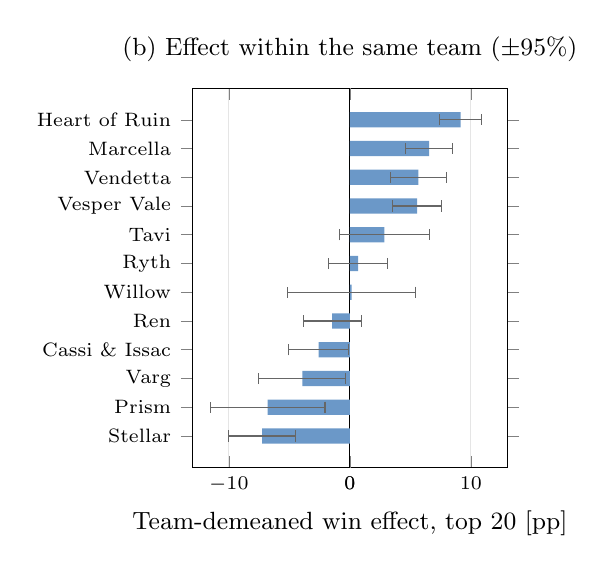
\begin{tikzpicture}
\begin{axis}[
  width=0.46\linewidth, height=6.4cm,
  xbar, bar width=5.5pt,
  xmin=-13, xmax=13,
  symbolic y coords={Stellar,Prism,Varg,CI,Ren,Willow,Ryth,Tavi,Vesper,Vendetta,Marcella,HoR},
  ytick=data, yticklabels={Stellar,Prism,Varg,Cassi \& Issac,Ren,Willow,Ryth,Tavi,Vesper Vale,Vendetta,Marcella,Heart of Ruin}, y tick label style={font=\scriptsize},
  xlabel={Team-demeaned win effect, top 20 [pp]},
  xmajorgrids, grid style={gray!20},
  tick label style={font=\scriptsize}, label style={font=\small},
  title={\small (b) Effect within the same team ($\pm$95\%)},
  extra x ticks={0}, extra x tick style={grid style={black, thin}}
]
\addplot[fill=cTop!70, draw=none, error bars/.cd, x dir=both, x explicit, error bar style={black!60}]
 coordinates {
 (-7.26,Stellar) +- (2.75,0)
 (-6.80,Prism) +- (4.74,0)
 (-3.93,Varg) +- (3.60,0)
 (-2.59,CI) +- (2.49,0)
 (-1.47,Ren) +- (2.40,0)
 (0.15,Willow) +- (5.27,0)
 (0.67,Ryth) +- (2.43,0)
 (2.85,Tavi) +- (3.71,0)
 (5.56,Vesper) +- (2.03,0)
 (5.65,Vendetta) +- (2.30,0)
 (6.54,Marcella) +- (1.95,0)
 (9.15,HoR) +- (1.75,0)
 };
\end{axis}
\end{tikzpicture}
\caption{Champion meta in the 10-21 dump. Top teams over-pick the champions that help (solid lines) and avoid those that hurt (dashed). Sources: \href{\scratch/matchdb/out/champ_stats.csv}{\texttt{champ\_stats.csv}}, \href{\scratch/matchdb/out/champ_team_demeaned.csv}{\texttt{champ\_team\_demeaned.csv}}.}
\label{fig:picks}
\end{figure}

\subsection{Drafts are a fixed function of the map, not of the opponent}

The current (10-22) top-20 drafts move the meta even further towards the core. In 165 top-10-vs-top-10 matches, Vesper Vale appears in \textbf{91\%} of team-games, Heart of Ruin in 85\%, Marcella 78\%, Vendetta 64\% and Ryth 56\%. Stellar and Ren were common on 10-21 (67 and 68 picks in 86 top-vs-top games) and now have \textbf{one pick each} \src{\scratch/top1-10/meta_top10.txt}{top1-10/meta\_top10.txt}. Ranks 11--20 look the same: Vesper 92\% of sides, Ryth 82\%, Marcella 80\% \src{\scratch/top11-20/cross.txt}{top11-20/cross.txt}. The timing matches the patch our own draft notes describe: Vesper, Vendetta, Tavi and Prism buffed; Stellar, Heart of Ruin and Ren nerfed \src{\repo/bots/bot-v5/src/draft.rs}{bot-v5/src/draft.rs:12}. The dump's verdict on Stellar and Ren therefore holds even more strongly now. The one-sided Heart of Ruin effect may have shrunk, though. When only one side had Heart of Ruin in top-10 games, that side won just 43\% (n = 42).

The structural finding is that \textbf{every top-10 team drafts deterministically by map}. Between 8 and 13 maps per team were played more than once, and none of them ever got two different drafts, whatever the opponent or side. The pick list is simply cut to the map's 3-, 4- or 5-champion size \src{\scratch/top1-10/drafts_by_team.txt}{top1-10/drafts\_by\_team.txt}. Nine of the ten teams at ranks 11--20 use one fixed list. NEETCoders and hello switch lists by map, and NEETCoders' C\&I/Stellar variant wins 65\% on the maps where it uses it. No team visibly counter-picks \src{\scratch/top11-20/lists_report.txt}{top11-20/lists\_report.txt}. Mirror picks are legal, so denying a champion gains nothing, and per-map tables are cheap because the draft bot sees the whole map.

\begin{table}[H]
\centering\small
\caption{Main 5-pick drafts of the top 10 on 10-22 (40 ranked games each) and the plan each one supports. Sources: \href{\scratch/top1-10/drafts_by_team.txt}{\texttt{drafts\_by\_team.txt}}, \href{\scratch/top1-10/agg_current.txt}{\texttt{agg\_current.txt}}.}
\begin{tabularx}{\linewidth}{@{}l r X X@{}}
\toprule
Team (rating) & Win\% & Main draft, in pick order & Win plan visible in the data\\
\midrule
1 Intercontinental Fish (2298) & 65 & Vesper, Vendetta, HoR, \CI, Ryth & Vesper hyper-carry: 49\% of team gold, ${\sim}$104 Power Strength shards per game\\
2 prism best girl (2235) & 65 & Prism, Vesper, Marcella, Ryth/Vendetta, HoR & Prism gem bank, Vesper + Marcella killers, Ryth stuns (11 assists per game)\\
3 procless (2169) & 52 & HoR, Vesper, Ryth, Marcella, Vendetta & Pure farming: Treasure-first, no locks, 5.0 kills per game\\
4 policy wonk (2139) & 65 & Marcella, Vesper, Tavi, Willow, Ryth & Marcella carry: 4,135 gold per game, Willow heals 12.5k\\
5 new team(4) (2126) & 55 & HoR, Marcella, Vesper, Ryth, Vendetta & Balanced; 13--4 on 3/4-pick maps\\
6 Univardisty of Shingtonwash (2118) & 42 & Marcella, Varg, HoR, Vendetta, Vesper & Shields (56.8k per game), 258 wards\\
7 :3 (2117) & 52 & HoR, Prism, Vendetta, Vesper, Marcella & Prism bank; opening hit hard by fuel exhaustion\\
8 Pantheon (2113) & 42 & Prism, Vesper, Marcella, Ryth/Vendetta, HoR & Fastest small tributes, biggest Prism bank\\
9 Sponge (2073) & 52 & HoR, Ryth, Vendetta, Willow, Marcella & HoR killer (244 kills in 40 games)\\
10 EMPEROR Tung (2049) & 40 & HoR, Vesper, Marcella, Ryth, Vendetta & Treasure-first farming, slowest gem curve\\
\bottomrule
\end{tabularx}
\label{tab:drafts}
\end{table}

%=====================================================================
\section{Ranks 1--3 win through execution rather than a shared trick}
%=====================================================================

\subsection{One game rhythm, three win plans}

Every top bot follows the same rhythm (Figure~\ref{fig:flow}). Champions split up and farm camps solo from about round 15--30, clearing 3.6--5.5 camps by round 100. On their first shop visit (round 40--84) they buy five shards at once, which completes a 150-gold emblem, usually Treasure (+20\% gold) or Jungle ($-$30\% camp damage). Fewer than one kill per game happens before round 100 \src{\scratch/top1-10/agg_current.txt}{top1-10/agg\_current.txt}. Nobody rushes. The 11--20 band does the same: Treasure, then Jungle, then Bruiser or Power stat emblems from about round 400 \src{\scratch/top11-20/agg_recent.txt}{top11-20/agg\_recent.txt}. The separation happens in the middle game. Ranks 1--3 have \textbf{394 gold at round 100 against 334} for ranks 8--10, and 2,670 against 2,367 at round 500, while holding opponents to 211 gems at round 500 against 253 \src{\scratch/top1-10/records.jsonl}{top1-10/records.jsonl}. Games end on the 1,000-gem race after a median of about 1,000--1,150 rounds (229 of 235).

\begin{figure}[H]
\centering
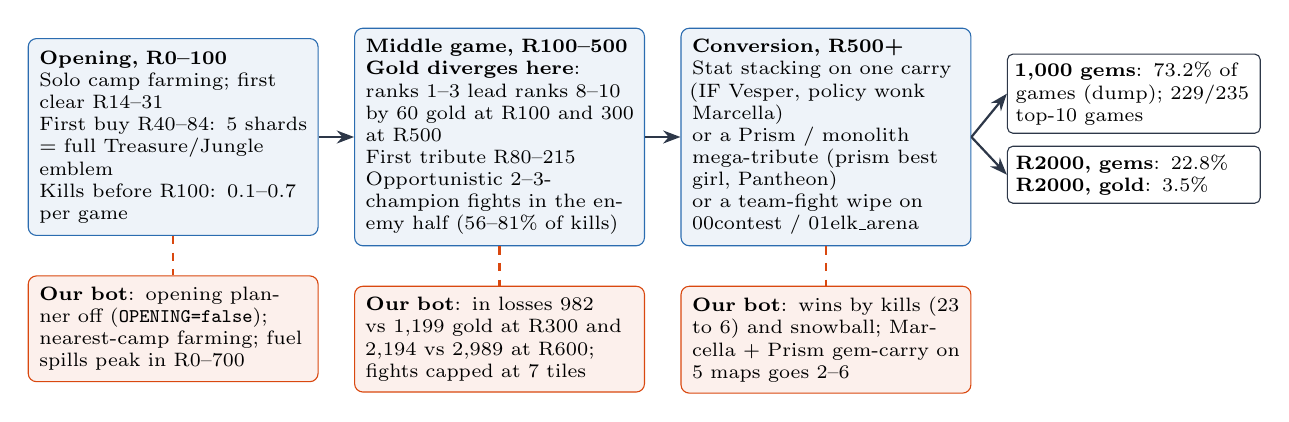
\begin{tikzpicture}[
  font=\scriptsize,
  phase/.style={draw=cTop, fill=cTop!8, rounded corners=3pt, text width=3.4cm, minimum height=2.5cm, align=left, inner sep=4pt},
  ours/.style={draw=cOurs, fill=cOurs!8, rounded corners=3pt, text width=3.4cm, align=left, inner sep=4pt},
  endn/.style={draw=cInk, fill=white, rounded corners=2pt, text width=3.0cm, align=left, inner sep=3pt},
  arr/.style={-{Stealth[length=2.2mm]}, thick, cInk}
]
\node[phase] (op) {\textbf{Opening, R0--100}\\Solo camp farming; first clear R14--31\\First buy R40--84: 5 shards = full Treasure/Jungle emblem\\Kills before R100: 0.1--0.7 per game};
\node[phase, right=0.45cm of op] (mid) {\textbf{Middle game, R100--500}\\\textbf{Gold diverges here}: ranks 1--3 lead ranks 8--10 by 60 gold at R100 and 300 at R500\\First tribute R80--215\\Opportunistic 2--3-champion fights in the enemy half (56--81\% of kills)};
\node[phase, right=0.45cm of mid] (late) {\textbf{Conversion, R500+}\\Stat stacking on one carry (IF Vesper, policy wonk Marcella)\\or a Prism / monolith mega-tribute (prism best girl, Pantheon)\\or a team-fight wipe on 00contest / 01elk\_arena};
\node[endn, right=0.45cm of late, yshift=0.55cm] (e1) {\textbf{1,000 gems}: 73.2\% of games (dump); 229/235 top-10 games};
\node[endn, below=0.15cm of e1] (e2) {\textbf{R2000, gems}: 22.8\%\\\textbf{R2000, gold}: 3.5\%};
\draw[arr] (op) -- (mid); \draw[arr] (mid) -- (late);
\draw[arr] (late.east) -- (e1.west); \draw[arr] (late.east) -- (e2.west);
\node[ours, below=0.5cm of op] (o1) {\textbf{Our bot}: opening planner off (\texttt{OPENING=false}); nearest-camp farming; fuel spills peak in R0--700};
\node[ours, below=0.5cm of mid] (o2) {\textbf{Our bot}: in losses 982 vs 1,199 gold at R300 and 2,194 vs 2,989 at R600; fights capped at 7 tiles};
\node[ours, below=0.5cm of late] (o3) {\textbf{Our bot}: wins by kills (23 to 6) and snowball; Marcella + Prism gem-carry on 5 maps goes 2--6};
\draw[cOurs, dashed, thick] (op.south) -- (o1.north);
\draw[cOurs, dashed, thick] (mid.south) -- (o2.north);
\draw[cOurs, dashed, thick] (late.south) -- (o3.north);
\end{tikzpicture}
\caption{The game rhythm shared by top-20 bots (blue) and where our bot departs from it (orange). End-condition shares are ladder-wide from the 10-21 dump. Sources: \href{\scratch/top1-10/agg_current.txt}{\texttt{top1-10/agg\_current.txt}}, \href{\scratch/matchdb/out/map_stats.csv}{\texttt{map\_stats.csv}}, \href{\scratch/ours/rows.json}{\texttt{ours/rows.json}}.}
\label{fig:flow}
\end{figure}

The three best teams then reach 1,000 gems in three different ways. \textbf{Intercontinental Fish} (\#1) puts everything into one ranged carry. Its Vesper Vale earns 3,696 gold per game, 49\% of the team's total, and turns about 3,100 gold of it into Power Strength. That Vesper gets 171 of the team's kills in 40 games. In every other top-10 team Vesper takes 19--37\% of the gold. IF has the fastest close-out of the ten (median 980 rounds in wins) \src{\scratch/top1-10/agg_current.txt}{top1-10/agg\_current.txt}. \textbf{prism best girl} (\#2) banks gems on Prism, which gains Focus for each gem carried. Its Prism carries 89.6 gems on average (median peak 216) and tributes only about half of what it collects. The team makes the fewest and largest tributes in the top 10 (75.3 gems on average), and Vesper and Marcella get 167 and 163 kills. \textbf{procless} (\#3) simply farms: 5.0 kills per game, Treasure-first builds on all five champions, no altar locks. \textbf{policy wonk} (\#4) is the clearest Marcella carry on the ladder. Marcella earns 4,135 gold per game and gets 2 gold per tributed gem, and the team has the ladder's highest gold at round 300 (1,557) and the most final gold (9,439). It converted all 14 of the games it led at round 500.

\subsection{Techniques that pay, and techniques that only look busy}

The summaries let us measure seven techniques. Not all of them correlate with rank (Table~\ref{tab:tech}). Altar locks are the clearest case. Ranks 2 and 3 never buy them. Ranks 5, 7, 8 and 9 buy 7.4--8.8 per game. Ranks 1--3 average 1.7 locks per game against 7.5 for ranks 8--10 \src{\scratch/top1-10/records.jsonl}{top1-10/records.jsonl}. In the 11--20 band PDI has the best record (61--39) and uses no consumables at all \src{\scratch/top11-20/lists_report.txt}{top11-20/lists\_report.txt}. A lock delays a tribute but does not stop it, since five attacks clear one. Vision is similar: Univardisty of Shingtonwash places the most wards (258 per game) and wins 42\%. Fast, small tributes are actively misleading. Pantheon has the best gems at rounds 100 and 300 (35/144) and still finishes with the second-lowest gold (5,372) and a 42\% record. In the 11--20 band, the gem-rushers Trzy Kwaterki and \#20 ({\jp ひななー}) are 4--11 and 5--10.

\begin{table}[H]
\centering\small
\caption{Measured techniques among the top 20 (10-22 data) and whether they separate ranks. Sources: \href{\scratch/top1-10/agg_current.txt}{\texttt{top1-10/agg\_current.txt}}, \href{\scratch/top1-10/records.jsonl}{\texttt{records.jsonl}}, \href{\scratch/top11-20/agg_recent.txt}{\texttt{top11-20/agg\_recent.txt}}.}
\begin{tabularx}{\linewidth}{@{}>{\raggedright}p{3.0cm} X >{\raggedright\arraybackslash}p{3.4cm}@{}}
\toprule
Technique & Evidence & Verdict\\
\midrule
Hyper-carry stat stacking & IF Vesper 104 Power Strength shards per game; policy wonk Marcella ${\sim}$102 Bruiser shards & \textcolor{cGood}{Pays}: ranks 1 and 4\\
Treasure-first emblem & procless, EMPEROR Tung, Sponge, policy wonk, IF; band teams that finish an emblem by R110--170 out-earn the others & \textcolor{cGood}{Pays}: shared by the top\\
Prism gem bank & prism best girl 89.6 gems carried on average; Pantheon's 737-gem single tribute (2822eea9) & \textcolor{cInk}{Mixed}: rank 2 but also rank 8 (42\%)\\
Monolith farming & prism best girl 28 camp pickups of 100+ gems (18 on 00contest), IF 16, Pantheon 0 & \textcolor{cGood}{Pays} on contest maps\\
Altar-lock spam & Ranks 1--3: 1.7 per game; ranks 8--10: 7.5 & \textcolor{cBad}{Does not separate}\\
Teleport-crystal spam & Ranks 1--3: 3.2 per game; ranks 8--10: 8.2 & \textcolor{cBad}{Does not separate}\\
Ward volume & UoS 258 per game at 42\%; LARP 17 per game & \textcolor{cBad}{Does not separate}\\
Willow sustain & policy wonk heals 12.5k per game; Noobot's Willow earns 132 gold per game & \textcolor{cInk}{Only with a carry}\\
\bottomrule
\end{tabularx}
\label{tab:tech}
\end{table}

\subsection{Faults at the top: blowouts, fuel and unbanked gems}

Top teams have faults too, and they are instructive. Losses come in two kinds. Close races are lost by one or two tributes. \textbf{Blowouts} (finishing under 300 gems) come from team-fight wipes on fight-heavy maps. IF is 0--2 on 01elk\_arena, including a 0--1,008 loss with 66 deaths to policy wonk (9fff921f). 00contest and 01elk\_arena produced 6 and 5 shutouts in the sample \src{\scratch/top1-10/records.jsonl}{top1-10/records.jsonl}. \textbf{:3} (\#7) has 199 fuel-exhaustion events per game, about 190 of them before round 250. It has the latest first tribute of the top 10 (median round 215) and still ranks 7th, which suggests it is strong later in the game. \textbf{Univardisty of Shingtonwash} ends games carrying 173 unbanked gems in its losses. Gem-stealing against bag carriers pays: UoS loses 85 gems per game on death and Pantheon 108. In the 11--20 band, \textbf{every team has 3--5 maps it goes 0--3 or worse on}. Examples are 01islands 0/12, 00expanse 2/10 and 01big\_world 3/13 against teams outside the band. Trzy Kwaterki (34 events per game) and Tartarus (9.1) are the only band teams with real fuel problems \src{\scratch/top11-20/agg_recent.txt}{top11-20/agg\_recent.txt}. No team in the top 20 crashed in any sampled game.

Robustness also tracks rank inside the top 10. Ranks 1--3 have essentially zero fuel events (0.1 per game, all of them procless), and ranks 8--10 average 6.6 \src{\scratch/top1-10/records.jsonl}{top1-10/records.jsonl}. When ranks 11--20 lose to the top 10, the gap is gold and kills, not gems: 795 against 1,078 gold at round 250, 1,679 against 2,760 at round 500, and 4.5 against 13.4 kills. In 13 of those 30 losses the band team \emph{led on gems at round 500} \src{\scratch/top11-20/cross.txt}{top11-20/cross.txt}. The top 10 don't win by tributing first. They win by building a gold and stat lead that turns into decisive fights, and then converting it.

%=====================================================================
\section{Our bot wins fights but loses farming races to its peers}
%=====================================================================

\subsection{A 66\% record that hides a 9--16 record against peers}

Our team, \emph{Anime girls against \#2 period cramp} (0d643742\ldots), went \textbf{33--17} in its last 50 ranked games on 10-22. The drafts carry the fingerprints of the v5 code: Marcella then Prism on all 8 gem-carry-map games, and Vesper in 47 of 50 rosters. The live bundle is most likely \code{bots/bot-v5/man.zip}{bots/bot-v5/man.zip}, which is source-identical to \code{\vfive}{bot-v5-r175199} \src{\scratch/ours/me_ranked.json}{ours/me\_ranked.json}. This is inferred from the drafts, because the CLI cannot list the active submission. The record splits sharply by opponent strength (Figure~\ref{fig:record}). Against the three teams just above us (Latent Tactics \#93, Zkey Farming \#94, will think later \#97) we went \textbf{5--10}. Against the five teams ranked \#123 and below we went \textbf{22--3}. Over the sample our rating fell from \#97 (1764.7) to \#108 (1748.5) \src{\scratch/ours/rows.json}{ours/rows.json}.

\begin{figure}[H]
\centering
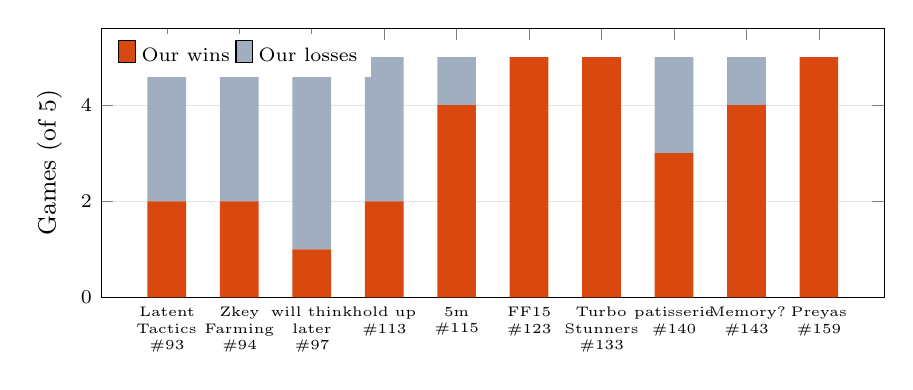
\begin{tikzpicture}
\begin{axis}[
  width=0.95\linewidth, height=5.0cm,
  ybar stacked, bar width=14pt,
  ymin=0, ymax=5.6, ylabel={Games (of 5)},
  symbolic x coords={LT,ZF,WTL,HU,5m,FF15,TS,PDPN,Mem,Prey},
  xtick=data,
  xticklabels={{Latent Tactics\\\#93},{Zkey Farming\\\#94},{will think later\\\#97},{hold up\\\#113},{5m\\\#115},{FF15\\\#123},{Turbo Stunners\\\#133},{patisserie\\\#140},{Memory?\\\#143},{Preyas\\\#159}},
  xticklabel style={font=\tiny, align=center, text width=1.4cm},
  legend style={font=\scriptsize, at={(0.01,0.98)}, anchor=north west, draw=none, legend columns=2},
  ymajorgrids, grid style={gray!20},
  tick label style={font=\scriptsize}, label style={font=\small},
]
\addplot[fill=cOurs, draw=none] coordinates {(LT,2)(ZF,2)(WTL,1)(HU,2)(5m,4)(FF15,5)(TS,5)(PDPN,3)(Mem,4)(Prey,5)};
\addlegendentry{Our wins}
\addplot[fill=cLow, draw=none] coordinates {(LT,3)(ZF,3)(WTL,4)(HU,3)(5m,1)(FF15,0)(TS,0)(PDPN,2)(Mem,1)(Prey,0)};
\addlegendentry{Our losses}
\end{axis}
\end{tikzpicture}
\caption{Our last 50 ranked games (10-22, engine 1.0.3), by opponent and the opponent's later ladder rank. We are around \#97--\#108. Source: \href{\scratch/ours/rows.json}{\texttt{ours/rows.json}}.}
\label{fig:record}
\end{figure}

\subsection{Losses are low-contact economy races decided before round 300}

Wins and losses look like two different games. In \textbf{wins} we average 23 kills to 6 and 12,314 gold to 5,297, and blowouts reach 50--0 kills (e44f7fbe, 00swirl). In \textbf{losses} we get 2 kills to 7, and 7 of the 17 losses had no kills by us at all. A typical example is 71b8dc63 (00split), 426 to 1,012 gems by round 716 with no kills on either side \src{\scratch/ours/rows.json}{ours/rows.json}. The gold gap in losses already exists at round 300 and keeps growing (Figure~\ref{fig:econ}a). Peers who avoid our fights simply out-farm us until they reach 1,000 gems. The teams that beat us all draft Marcella and/or Vesper, and the strongest of them (Latent Tactics and Zkey Farming: Marcella, Vesper, Tavi, Willow, Ryth) get far more out of Marcella and Ryth than we do. Zkey's Marcella earned 3,088 gold and Ryth 2,114 in 71b8dc63. Latent's Marcella earned 4,688 in 1ec4d876. In those games our Ryth earned 180, 40 and 1,120 gold.

\begin{figure}[H]
\centering
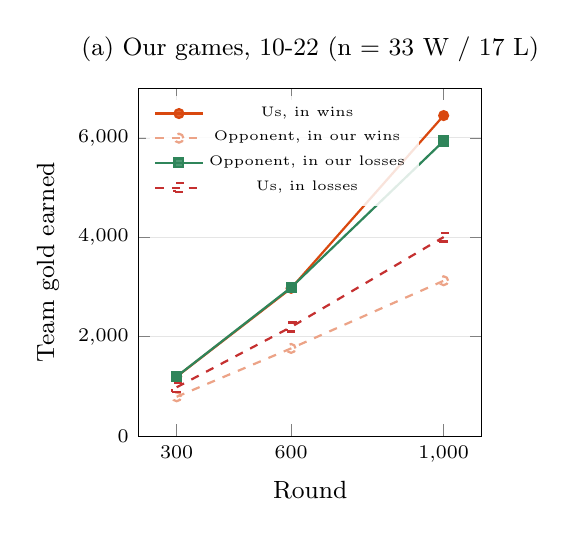
\begin{tikzpicture}
\begin{axis}[
  width=0.49\linewidth, height=6.0cm,
  xlabel={Round}, ylabel={Team gold earned},
  xtick={300,600,1000}, xmin=200, xmax=1100, ymin=0, ymax=7000,
  ymajorgrids, grid style={gray!20},
  tick label style={font=\scriptsize}, label style={font=\small},
  legend style={font=\tiny, at={(0.02,0.98)}, anchor=north west, draw=none, fill=white, fill opacity=0.85, text opacity=1},
  every axis plot/.append style={thick, mark size=1.6pt},
  title={\small (a) Our games, 10-22 (n = 33 W / 17 L)}
]
\addplot[cOurs, mark=*] coordinates {(300,1195)(600,2973)(1000,6449)}; \addlegendentry{Us, in wins}
\addplot[cOurs!50, mark=o, dashed] coordinates {(300,790)(600,1764)(1000,3125)}; \addlegendentry{Opponent, in our wins}
\addplot[cOpp, mark=square*] coordinates {(300,1199)(600,2989)(1000,5937)}; \addlegendentry{Opponent, in our losses}
\addplot[cBad, mark=square, dashed] coordinates {(300,982)(600,2194)(1000,4004)}; \addlegendentry{Us, in losses}
\end{axis}
\end{tikzpicture}\hfill
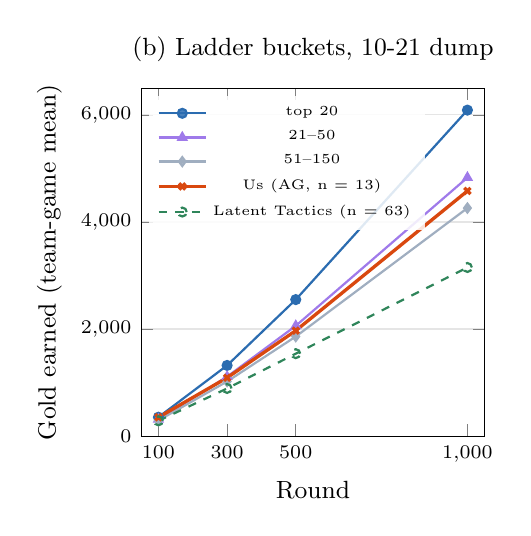
\begin{tikzpicture}
\begin{axis}[
  width=0.49\linewidth, height=6.0cm,
  xlabel={Round}, ylabel={Gold earned (team-game mean)},
  xtick={100,300,500,1000}, xmin=50, xmax=1050, ymin=0, ymax=6500,
  ymajorgrids, grid style={gray!20},
  tick label style={font=\scriptsize}, label style={font=\small},
  legend style={font=\tiny, at={(0.02,0.98)}, anchor=north west, draw=none, fill=white, fill opacity=0.85, text opacity=1},
  every axis plot/.append style={thick, mark size=1.6pt},
  title={\small (b) Ladder buckets, 10-21 dump}
]
\addplot[cTop, mark=*] coordinates {(100,353)(300,1320)(500,2550)(1000,6090)}; \addlegendentry{top 20}
\addplot[cMid, mark=triangle*] coordinates {(100,312)(300,1110)(500,2060)(1000,4830)}; \addlegendentry{21--50}
\addplot[cLow, mark=diamond*] coordinates {(100,292)(300,1020)(500,1860)(1000,4260)}; \addlegendentry{51--150}
\addplot[cOurs, mark=x, very thick] coordinates {(100,351)(300,1090)(500,1970)(1000,4580)}; \addlegendentry{Us (AG, n = 13)}
\addplot[cOpp, mark=o, dashed] coordinates {(100,285)(300,890)(500,1540)(1000,3150)}; \addlegendentry{Latent Tactics (n = 63)}
\end{axis}
\end{tikzpicture}
\caption{Economy curves. (a) In our losses the opponent leads by about 200 gold at round 300 and by almost 2,000 at round 1,000. In our wins the picture reverses. (b) On the older 10-21 build we kept pace with the top 20 up to round 100 (351 against 353) and then fell to the 21--50 level by round 300. Our dump sample is small (13 games). Sources: \href{\scratch/ours/rows.json}{\texttt{ours/rows.json}}, \href{\scratch/matchdb/out/profiles.csv}{\texttt{profiles.csv}}.}
\label{fig:econ}
\end{figure}

Figure~\ref{fig:econ}b gives the ladder-wide context on the older build, and it points to the same window. We open as fast as the top 20 (351 gold at round 100 against 353). By round 300 the gap is 230 gold (1,090 against 1,320), and by round 1,000 it is 1,510. Our first tribute came late (median round 216 against 118 for every bucket) \src{\scratch/matchdb/out/profiles.csv}{profiles.csv}. A late first tribute is not a fault in itself, because NTU banks until round 224 and has the band's best gold. Combined with the lower gold, though, it says our rounds 100--300 are less productive. Throughput is not the problem: we clear \emph{more} camps than the top 20 (78.8 against 59.6 per game in the dump, and 56 against 48 in our current losses). The problem is value per action: low-value camps, gems carried instead of tributed, and gold that turns into gems too slowly. In two losses we had more gold and still lost the gem race (bb3b6b4b 8,063 to 7,160 gold, 738 to 1,019 gems; 946c9409). The \code{bots/bot-v5/src/common/press.rs}{press.rs:1-6} comment describes the same failure on 00lanes, and its proposed fix is switched off (\texttt{PRESS=false}).

\subsection{The gem-carry draft and three map-specific failures}

The \textbf{Marcella + Prism gem-carry plan}, triggered by \code{\vfive/common/gemcarry.rs}{gemcarry.rs:23,61} through \code{\vfive/draft.rs}{draft.rs:248}, is \textbf{2--6} on 00gem\_fields, 00quadrants, 00lost\_world, 00great\_wall and 00road\_of\_riches. On all other maps we are 31--11. 00great\_wall alone is 0--3 \src{\scratch/ours/rows.json}{ours/rows.json}. Prism has the worst survival on our team (2.8 deaths per game, 7 wins in 17 games). In b6f381da it earned 40 gold in 864 rounds. The code's own test notes report 43--53 and 49--47 in the first trials and 8/12 on one seed afterwards. It was enabled because ``the top ladder team plays it'' \src{\repo/\vfive/common/gemcarry.rs}{gemcarry.rs:12-23}. The ladder agrees with the test notes rather than with the decision. Prism's top-20 team-demeaned effect is $-$6.8pp. Of the two top-10 teams that build around Prism, one (Pantheon) wins 42\%. prism best girl's version works because its Prism hoards safely for hundreds of rounds and tributes huge bags. Ours dies.

Three map-specific failures stand out. On \textbf{01boss\_battle}, in 3bca78ca we carried about 2,390 gems to round 2,000 and tributed none. We won only on the gold tiebreak, 26,552 to 14,777. In two other games Vesper made a single tribute of more than 1,200 gems at about round 1,460. The code marks this map's only altar as enclosed (\code{\vfive/common/base.rs}{base.rs:69-81}, \texttt{OPEN\_ALTARS\_ONLY}) \src{\scratch/ours/sum/}{ours/sum/3bca78ca}. On \textbf{01islands} (1--2), champions without a dash sit idle. In 1ec4d876 Stellar and Tavi ended with 0 gems over 1,127 rounds, and in c7a67204 Tavi's last gold came at round 426. A comment at \code{\vfive/common/collect.rs}{collect.rs:1178} already notes non-dashers ``hitting camps across holes''. On \textbf{00stampede} (59cf7d77) we had 32 deaths against 6 kills, and three champions collected 0 gems. We also lost both 00expanse games 0--0 on kills (about 500 to 1,030 gems), which looks like a pure farming race lost. The top-20 band is weak on several of these maps too (01islands 0/12, 00expanse 2/10), so per-map work here is shared ladder-wide value, not only our bug.

%=====================================================================
\section{Fuel exhaustion costs us about one turn in twelve}
%=====================================================================

There are \textbf{no crashes} in any of our 63 platform summaries, and no bot faults in local runs. The real fault is fuel. A \texttt{fuelExhausted} event fires on \textbf{8.6\% of our champion-turns} against 0.5\% for our opponents in the same games. That is about \textbf{570 lost turns per match}, ranging from 57 to 2,480 \src{\scratch/ours/sum/}{ours/sum, an3.py}. The rules say a bot that runs out of fuel is suspended and resumes only the next round \src{\repo/docs/GameRules.md}{GameRules.md:335-345}. The team's own notes call this effectively a lost turn \src{\repo/docs/RustFuelPitfalls.md}{docs/RustFuelPitfalls.md}. Every champion is affected: Heart of Ruin averages 191 exhaustions per champion-game, Vesper 105. The rate reproduces locally (release build 8.3\% and 7.3\% in a mirror match). The 10-21 bot had the same rate (0.079), so the problem is chronic rather than a v5 regression. Figure~\ref{fig:fuel}a puts this on a log scale against the ladder.

\begin{figure}[H]
\centering
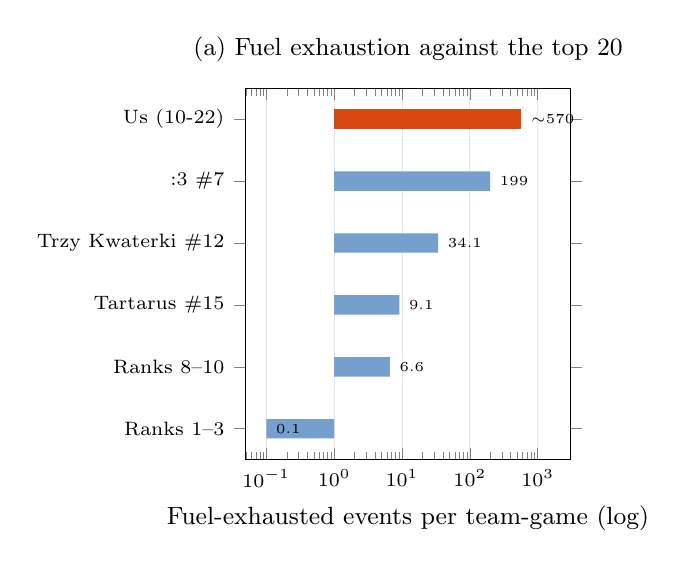
\begin{tikzpicture}
\begin{axis}[
  width=0.47\linewidth, height=6.3cm,
  xbar, bar width=7pt, xmode=log, log basis x=10,
  xmin=0.05, xmax=3000,
  symbolic y coords={r13,r810,tar,tk,c3,us},
  ytick={r13,r810,tar,tk,c3,us}, yticklabels={Ranks 1--3,Ranks 8--10,Tartarus \#15,Trzy Kwaterki \#12,:3 \#7,Us (10-22)}, bar shift=0pt, y tick label style={font=\scriptsize},
  xlabel={Fuel-exhausted events per team-game (log)},
  xmajorgrids, grid style={gray!20},
  tick label style={font=\scriptsize}, label style={font=\small},
  nodes near coords, nodes near coords style={font=\tiny, anchor=west},
  point meta=explicit symbolic,
  title={\small (a) Fuel exhaustion against the top 20}
]
\addplot[fill=cTop!65, draw=none] coordinates {(0.1,r13)[0.1] (6.6,r810)[6.6] (9.1,tar)[9.1] (34.1,tk)[34.1] (199,c3)[199]};
\addplot[fill=cOurs, draw=none] coordinates {(570,us)[${\sim}$570]};
\end{axis}
\end{tikzpicture}\hfill
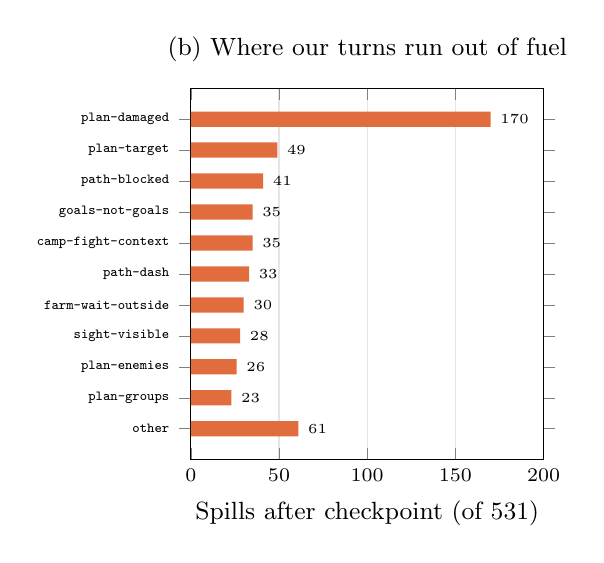
\begin{tikzpicture}
\begin{axis}[
  width=0.50\linewidth, height=6.3cm,
  xbar, bar width=5.5pt,
  xmin=0, xmax=200,
  symbolic y coords={other,plan-groups,plan-enemies,sight-visible,farm-wait-outside,path-dash,camp-fight-context,goals-not-goals,path-blocked,plan-target,plan-damaged},
  ytick=data, y tick label style={font=\tiny\ttfamily},
  xlabel={Spills after checkpoint (of 531)},
  xmajorgrids, grid style={gray!20},
  tick label style={font=\scriptsize}, label style={font=\small},
  nodes near coords, nodes near coords style={font=\tiny},
  title={\small (b) Where our turns run out of fuel}
]
\addplot[fill=cOurs!80, draw=none] coordinates {(61,other)(23,plan-groups)(26,plan-enemies)(28,sight-visible)(30,farm-wait-outside)(33,path-dash)(35,camp-fight-context)(35,goals-not-goals)(41,path-blocked)(49,plan-target)(170,plan-damaged)};
\end{axis}
\end{tikzpicture}
\caption{(a) Our fuel exhaustion is about three times that of :3, the worst top-10 offender, and three to four orders of magnitude above ranks 1--3. (b) A traced local 600-round 00great-wall mirror (debug build, 531 spills). The checkpoint after which each spill happened is almost always inside the farm planner. ``other'' is the remainder of the 531. Sources: \href{\scratch/top1-10/records.jsonl}{\texttt{top1-10/records.jsonl}}, \href{\scratch/top11-20/agg_recent.txt}{\texttt{top11-20/agg\_recent.txt}}, \texttt{scratchpad/scripts/spill.py}.}
\label{fig:fuel}
\end{figure}

The trace points at three code sites. The first is \textbf{the farm planner} \code{\vfive/common/farm.rs}{farm.rs:835} (\texttt{farm\_plan}), with checkpoints at lines 868, 954, 1644, 1821, 1935 and 1975. \texttt{plan-groups} costs 19k fuel on average, \texttt{plan-target} 13k and \texttt{plan-rally-decision} 11k. The second is \textbf{the camp-fight context} at \code{\vfive/common/collect.rs}{collect.rs:341} (14k on average). The third is \textbf{the per-turn sight rebuild} at \code{\vfive/common/world.rs}{world.rs:47-75}. On round 2 alone, \texttt{sight-camps} costs 58k and \texttt{plan-enemies} 54k. The source already contains the diagnosis: turns ``reached the farm step with $\sim$82k fuel and a plan cost 50--90k''. Raising \texttt{FARM\_PLAN\_MIN\_FUEL} to 85k cut exhaustion by only 17\% \src{\repo/\vfive/common/farm.rs}{farm.rs:2150-2159}. Figure~\ref{fig:budget} shows why a threshold cannot fix it. The guard compares the fuel left against a fixed number, but the plan's cost varies by 40k from turn to turn. The beat pattern in the event log fits this: Ryth runs out every 3 rounds in 3bca78ca (12, 15, 18, 21, \ldots) and Tavi every 2 rounds in a0668720. That is what happens when a plan is cut off, finished on the next turn, and rebuilt (\texttt{STALE\_PLAN\_ROUNDS=3}).

\begin{figure}[H]
\centering
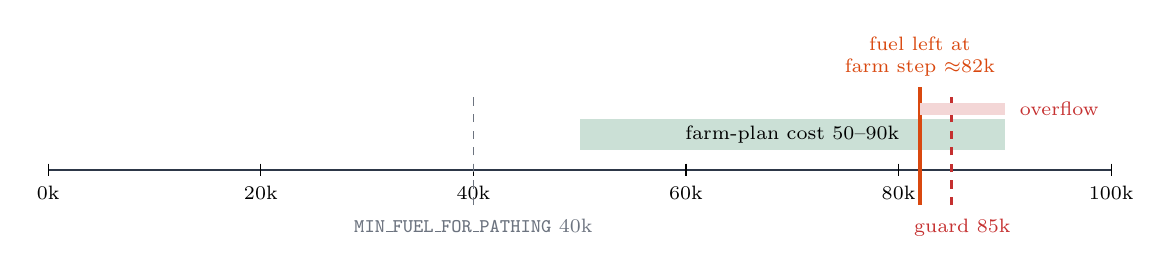
\begin{tikzpicture}[x=0.135cm, y=1cm, font=\scriptsize]
\draw[thick, cInk] (0,0) -- (100,0);
\foreach \v in {0,20,40,60,80,100} {\draw (\v,0.08) -- (\v,-0.08) node[below] {\v k};}
\fill[cOpp!25] (50,0.25) rectangle (90,0.65);
\node at (70,0.45) {farm-plan cost 50--90k};
\draw[cOurs, very thick] (82,-0.45) -- (82,1.05) node[above, align=center] {fuel left at\\farm step $\approx$82k};
\draw[cBad, very thick, dashed] (85,-0.45) -- (85,0.95);
\node[cBad, anchor=north] at (86,-0.5) {guard 85k};
\draw[cInk!70, dashed] (40,-0.45) -- (40,0.95);
\node[cInk!70, anchor=north] at (40,-0.5) {\texttt{MIN\_FUEL\_FOR\_PATHING} 40k};
\fill[cBad!20] (82,0.7) rectangle (90,0.85);
\node[cBad, anchor=west] at (90.5,0.78) {overflow};
\end{tikzpicture}
\caption{Why a fixed fuel guard leaks. A plan that costs more than the fuel left (red band) suspends the champion until the next round. The guard at 85k sits inside the plan's 40k cost range, so it can only trade lost turns for stale plans. Values from the comments and constants in \code{\vfive/common/farm.rs}{farm.rs:2150-2159} and \code{\vfive/bot.rs}{bot.rs:8}.}
\label{fig:budget}
\end{figure}

How much this costs us in rating is uncertain. In the dump, ranks 51--150 teams with more than 500 exhausted turns per game score \textbf{$-$10.3pp} against Elo (n = 75), compared with $-$1.3pp for teams with none. A few top-20 teams with heavy exhaustion score \emph{positive}, presumably because their compute is heavy by design \src{\scratch/matchdb/out/analysis2.txt}{matchdb/out/analysis2.txt}. Both figures are correlations. The mechanism is not in doubt, though. Losing about 9\% of turns slows farming, banking and fighting together, and peak exhaustion falls in rounds 0--700, the same window in which Section 1 shows games are decided. :3 shows the scale of the upside: it ranks 7th despite losing much of its first 250 rounds this way.

%=====================================================================
\section{What the top teams do better than us}
%=====================================================================

Table~\ref{tab:gap} sets the measurable differences side by side. Three of them are about converting the economy, not about skill in fights. The top 20 die less, earn more gold per action, and keep every turn. Kills are the one area where we already match or beat them (13.5 against 11.6 kills per game in the dump). That is why we beat weaker teams so easily, and why the strength doesn't carry over against peers who refuse to fight.

\begin{table}[H]
\centering\small
\caption{Top 20 versus our team. ``Dump'' figures are 10-21 team-game means (our n = 13, older build). ``Current'' figures are from 10-22. Sources: \href{\scratch/matchdb/out/profiles.csv}{\texttt{profiles.csv}}, \href{\scratch/top1-10/agg_current.txt}{\texttt{top1-10/agg\_current.txt}}, \href{\scratch/ours/rows.json}{\texttt{ours/rows.json}}.}
\begin{tabularx}{\linewidth}{@{}>{\raggedright\arraybackslash}p{4.4cm} >{\raggedright\arraybackslash}p{2.5cm} >{\raggedright\arraybackslash}p{2.7cm} X@{}}
\toprule
Metric & Top 20 & Us & What it tells us\\
\midrule
Gold earned by R100 (dump) & 353 & 351 & The opening is fine\\
Gold earned by R300 (dump) & 1,320 & 1,090 & The gap opens in rounds 100--300\\
Gold by R300, current losses & -- & 982 vs 1,199 & Peers out-farm us early\\
Gems tributed by R1000 (dump) & 621 & 502 & Slower conversion\\
Deaths per game (dump) & 7.2 & 10.4 & Better than mid-ladder (15.2), not top level\\
Kills per game (dump) & 11.6 & 13.5 & Our edge, but it doesn't win races\\
Camp clears per game (dump) & 59.6 & 78.8 & More actions, less value per action\\
Team-games with any fuel exhaustion (dump) & 37.9\% & 100\% & Chronic, every game\\
Fuel events per game, current & ranks 1--3: 0.1 & ${\sim}$570 & Largest single fault\\
Draft & fixed core, set per map & Vesper core + gem-carry swap & Our map rule picks a losing plan (2--6)\\
Win plan & one clear carry or bank & fight snowball & No plan against low-contact peers\\
\bottomrule
\end{tabularx}
\label{tab:gap}
\end{table}

Some strengths of ours should be kept. Our first-100-round gold matches the top 20. We have no crashes. We kill more than the top-20 average, and our camp throughput is the highest of any group measured. The fight engagement rules (capped at 7 tiles at \code{\vfive/common/fight.rs}{fight.rs:21}; enemies standing on their own spawn ignored at \code{\vfive/common/fight.rs}{fight.rs:17}) don't look like the cause of our losses. The cause is that low-contact opponents never come into range. The open question is whether we should go and find them. The top teams' kills fall 56--81\% in the enemy half, with about two assisters per kill, which suggests coordinated pick-offs of enemy farmers. The 11--20 band, on the other hand, gets run over when it fights in the enemy half (69\% of its deaths against the top 10 come in its own half, after it has fallen behind). The summaries cannot settle which applies to us, so invasion should be tested rather than assumed.

%=====================================================================
\section{What the replays show: top teams invade together, we stand still}
\label{sec:replays}
%=====================================================================

The summaries record totals and events but not where champions are on each turn. To fill that gap we decoded full replays with the engine build that ships inside the \texttt{cambc} visualiser (Appendix~\ref{app:replays}). The sample is every game in part 1 of the 10-21 replay dump that involves our team (13), two top-20 teams (1,131), or a top-20 team against a team ranked \#76--115 (601): 1,745 games and 3,490 team-games. These are the \emph{previous day's} bots, before the draft shift, so the numbers describe behaviour styles rather than today's exact rosters \src{\viz/an/features.jsonl}{features.jsonl}, \src{\viz/an/compare.py}{compare.py}.

\subsection{Top teams take the fight to weaker teams' half}

Figure~\ref{fig:invade} shows the clearest pattern. When a top-20 team meets a team ranked \#76--115, the top team spends about \textbf{21\%} of its champion-rounds in the enemy half and the lower team only \textbf{11\%}. The lower team dies \textbf{19.1} times a game against the top team's 3.9--6.1, and only \textbf{25\%} of its deaths happen in the enemy half. In other words, teams in our band are not losing fights they start. They are being farmed at home. The top teams also tribute in bigger batches (49--58 gems per tribute against 34.5) and reach 217--283 gems by round 500 against 141.

\begin{figure}[H]
\centering
\begin{minipage}{0.48\linewidth}\centering
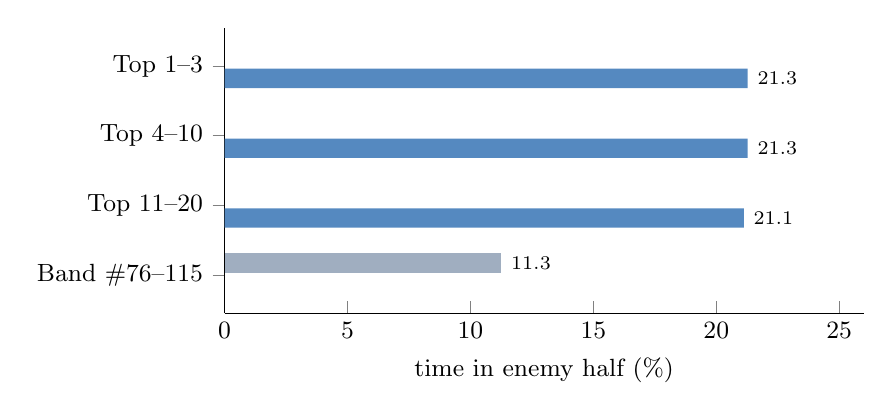
\begin{tikzpicture}
\begin{axis}[xbar, width=0.8\linewidth, height=5.2cm, bar width=7pt, xmin=0, xmax=26,
  symbolic y coords={band,t3,t2,t1}, ytick={band,t3,t2,t1}, yticklabels={Band \#76--115,Top 11--20,Top 4--10,Top 1--3},
  xlabel={\small time in enemy half (\%)}, nodes near coords, nodes near coords style={font=\scriptsize},
  every node near coord/.append style={/pgf/number format/fixed,/pgf/number format/precision=1},
  tick label style={font=\small}, axis x line*=bottom, axis y line*=left, enlarge y limits=0.18]
\addplot[fill=cTop!80, draw=none] coordinates {(21.28,t1) (21.28,t2) (21.12,t3)};
\addplot[fill=cLow, draw=none] coordinates {(11.26,band)};
\end{axis}
\end{tikzpicture}
\end{minipage}\hfill
\begin{minipage}{0.48\linewidth}\centering
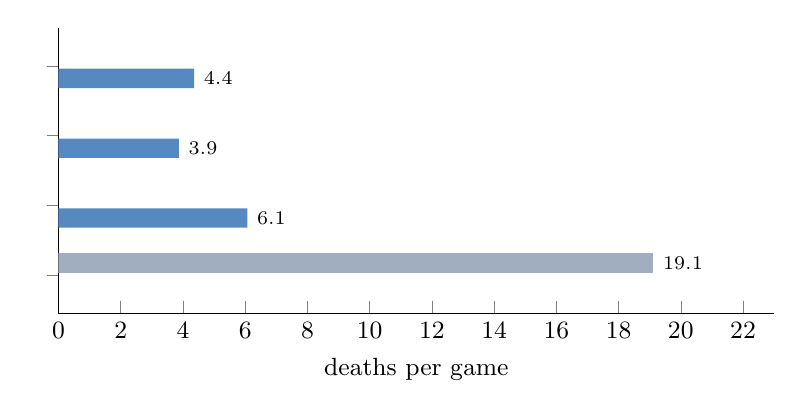
\begin{tikzpicture}
\begin{axis}[xbar, width=0.88\linewidth, height=5.2cm, bar width=7pt, xmin=0, xmax=23,
  symbolic y coords={band,t3,t2,t1}, ytick={band,t3,t2,t1}, yticklabels={},
  xlabel={\small deaths per game}, nodes near coords, nodes near coords style={font=\scriptsize},
  every node near coord/.append style={/pgf/number format/fixed,/pgf/number format/precision=1},
  tick label style={font=\small}, axis x line*=bottom, axis y line*=left, enlarge y limits=0.18]
\addplot[fill=cTop!80, draw=none] coordinates {(4.36,t1) (3.87,t2) (6.07,t3)};
\addplot[fill=cLow, draw=none] coordinates {(19.12,band)};
\end{axis}
\end{tikzpicture}
\end{minipage}
\caption{Head-to-head games between a top-20 team and a team ranked \#76--115 (601 games, 10-21 replays). The top team wins 81--97\% of them. Left: share of alive champion-rounds spent closer to the enemy's spawn than to one's own. Right: deaths per game; 75\% of the lower team's deaths are in its own half.}
\label{fig:invade}
\end{figure}

\subsection{How our bot moves compared with the top 20}

Table~\ref{tab:replay} compares the groups across all decoded games. Most fighting habits are similar everywhere: focus fire (84--90\% of rounds with several attacks hit one target), retreating at low health (39--47\%) and the first shop visit (round 61--69) barely vary. Our bot (13 games, 10-21 build) stands out in five places. It \textbf{stands still on 45\% of its alive rounds}, more than any top-20 team (30--42\%). It makes the fewest moves and casts the fewest abilities. It brings the fewest teammates to a kill. It loses the most carried gems when champions die. And it runs out of fuel on about \textbf{650 turns a game}, matching the 10-22 summaries, so the fuel fault predates v5.

\begin{table}[H]
\centering\small
\caption{Replay-measured behaviour, team-game means over all 1,745 decoded 10-21 games. ``Band'' rows are teams ranked \#76--115 and appear only as top-20 opponents. ``Still'' means the same tile as the previous round. Source: \href{\viz/an/compare.py}{\texttt{compare.py}} over \href{\viz/an/features.jsonl}{\texttt{features.jsonl}}.}
\begin{tabularx}{\linewidth}{@{}>{\raggedright\arraybackslash}X rrrrr@{}}
\toprule
Metric & Top 1--3 & Top 4--10 & Top 11--20 & Band & Us\\
\midrule
Team-games & 541 & 1,002 & 1,320 & 601 & 13\\
Win rate & 0.76 & 0.59 & 0.50 & 0.11 & 0.69\\
Standing still (\% of alive rounds) & 36.9 & 37.2 & 33.4 & 34.6 & \textbf{45.0}\\
Time in enemy half (\%) & 19.4 & 19.1 & 18.3 & 11.3 & 19.7\\
Ally within 4 tiles (\%) & 54.1 & 48.1 & 48.9 & 56.4 & 50.6\\
Moves per 100 alive rounds & 62.8 & 62.2 & 66.0 & 64.9 & \textbf{54.2}\\
Ability casts per 100 alive rounds & 11.8 & 10.6 & 10.0 & 10.3 & \textbf{8.9}\\
Teammates within 6 tiles of each kill & 1.79 & 1.74 & 1.62 & 1.55 & \textbf{1.34}\\
Deaths per game & 7.0 & 7.8 & 9.8 & 19.1 & 10.4\\
Gems lost on death per game & 83 & 93 & 81 & 112 & \textbf{131}\\
Gems per tribute & 48.2 & 46.3 & 41.2 & 34.5 & 34.5\\
Out-of-fuel turns per game & 0.2 & 113.5 & 16.1 & 21.3 & \textbf{654.5}\\
\bottomrule
\end{tabularx}
\label{tab:replay}
\end{table}

\subsection{Signature techniques visible only in replays}

\begin{itemize}[leftmargin=1.2em, itemsep=0.3em]
\item \textbf{Intercontinental Fish (\#1) moves as a pack.} A teammate is within 4 tiles on \textbf{66\%} of its champion-rounds, against 39--57\% for most of the top 20 (only Noobot, at 71\%, is clearly higher). It has zero out-of-fuel turns and buys no altar locks, and wins 85\% of its 264 decoded games.
\item \textbf{Pantheon (\#5) keeps a recall running.} Its champions cancel a recall at the start of each turn, act, then start a new recall at the end of the turn: about \textbf{4,500 recalls per game}, one per champion turn. Because damage interrupts a recall, this works as a tripwire. We think it is either a damage alarm or a fallback that walks the champion home if the bot fails to act, but the replay shows the pattern, not the intent. :3 (\#8) does something similar on a smaller scale (about 760 recalls per game).
\item \textbf{Fuel is not fatal on its own.} :3 loses about 550 turns a game to fuel and still wins 65\%, so fixing our fuel spill is necessary but not enough by itself.
\end{itemize}

\subsection{Case studies}

\textbf{A top-vs-top race: Intercontinental Fish 1,002--974 procless (055608db, 10-21).} Both teams tributed 30 gems by round 100, and Fish led for almost all of the rest of the game. Table~\ref{tab:case} shows the shape. For the first 300 rounds neither team went into the other's half. Fish then pushed in during rounds 500--699 (41--45\% of its champion-rounds in procless's half), and all three procless deaths in that stretch happened in procless's own half. The game was decided by steady banking plus one well-timed invasion, with no out-of-fuel turns on either side.

\textbf{Our worst loss: 0--1,008 against \#303 Feral Monoliths (0bd85570, 10-21).} Our champions held \textbf{zero gems at any point} in 1,535 rounds and never more than about 230 gold. At round 231 all five opponents collected gems together at the same central tiles (around 23--27, 22--26). That is a shared central gem camp our bot never contested. We also stood still on 37--57\% of alive rounds in every window and lost 820 turns to fuel.

\textbf{Current build on 01islands (1ec4d876, 10-22, engine 1.0.3).} Our five champions never got past about y = 44 on the 60-by-60 map, while the opponent's crossed the whole map. Tavi stood on one tile for \textbf{176 rounds}, and Stellar and Vendetta for 124 each; the opponent's longest stay was 21. Ren spent 244 rounds dead. This confirms recommendation~6: the champions are confined, not just idle.

\begin{table}[H]
\centering\small
\caption{Cumulative gems tributed by window end, and deaths, in the two 10-21 case studies. An asterisk marks a death in the enemy half. Source: \href{\viz/an/story.py}{\texttt{story.py}}.}
\begin{tabular}{@{}l rr l l@{\hspace{2em}} l rr@{}}
\toprule
\multicolumn{5}{c}{Fish (A) vs procless (B), 055608db} & \multicolumn{3}{c}{Us (A) vs Feral Monoliths (B), 0bd85570}\\
\cmidrule(r){1-5}\cmidrule(l){6-8}
Rounds & A & B & A deaths & B deaths & Rounds & A & B\\
\midrule
0--199 & 148 & 118 & 2 & 0 & 0--299 & 0 & 72\\
200--399 & 354 & 266 & 0 & 1 & 300--599 & 0 & 216\\
400--599 & 532 & 442 & 1 & 2 (1*) & 600--899 & 0 & 432\\
600--799 & 768 & 708 & 0 & 2 & 900--1199 & 0 & 720\\
800--983 & 1,002 & 974 & 2 & 3 (1*) & 1200--1535 & 0 & 1,008\\
\bottomrule
\end{tabular}
\label{tab:case}
\end{table}

%=====================================================================
\section{Recommended changes, in priority order}
%=====================================================================

Each recommendation lists its evidence and the code to change. Items 1--3 attack the round-100-to-500 economy gap, which decides most games.

\begin{enumerate}[leftmargin=1.4em, itemsep=0.45em]
\item \textbf{Remove the farm-planner fuel spills (largest expected gain).} \emph{Evidence:} 8.6\% of turns lost, against 0.5\% for our opponents and about 0 for ranks 1--3. It happens every game, peaks in rounds 0--700, and reproduces locally. The 10-21 replays show the same fault in the previous build (about 650 out-of-fuel turns a game), alongside the highest standing-still rate of any group (45\%); whether the two are linked is the first thing to check. \emph{Change:} make \texttt{farm\_plan} (\code{\vfive/common/farm.rs}{farm.rs:835}) resumable or incremental across turns. Cache \texttt{plan-groups} and \texttt{plan-target} results between rounds instead of rebuilding them every \texttt{STALE\_PLAN\_ROUNDS}. Replace the fixed \texttt{FARM\_PLAN\_MIN\_FUEL} guard (\code{\vfive/common/farm.rs}{farm.rs:2156}) with a check on fuel actually left before each costly sub-step. Cut the per-turn sight rebuild (\code{\vfive/common/world.rs}{world.rs:47-75}) and the camp-fight context (\code{\vfive/common/collect.rs}{collect.rs:341}) to incremental updates. Check new \texttt{Bitboard} allocations in these loops, at about 2k fuel each (\code{docs/RustFuelPitfalls.md}{RustFuelPitfalls.md}). \emph{Target:} under 0.5\% of turns in the local 00great-wall mirror, measured with the existing \texttt{spill.py}.

\item \textbf{Retire or gate the Marcella + Prism gem-carry draft.} \emph{Evidence:} 2--6 on the maps where it fires against 31--11 elsewhere. Prism has 2.8 deaths per game. Its own trials were near 50\%. Prism is $-$6.8pp in the top 20. \emph{Change:} disable \texttt{gemcarry::draft\_pick} (\code{\vfive/common/gemcarry.rs}{gemcarry.rs:23,61}; \code{\vfive/draft.rs}{draft.rs:248}) and fall back to the standard Vesper/Marcella core on those five maps. If gem-carry is kept, Prism must survive for hundreds of rounds before tributing, as it does for prism best girl. Our version does not do that today.

\item \textbf{Close the gold gap in rounds 100--300.} \emph{Evidence:} even with our opponents at round 100, then 230 gold behind the top 20 by round 300. In current losses we are 217 behind peers at round 300. A 300-gold deficit at round 300 wins only 16\% of games. Every top team buys a complete Treasure or Jungle emblem on its first shop visit (round 40--84) and rides one carry. \emph{Change:} enable and tune the opening planner (\code{\vfive/opening.rs}{opening.rs:35}, \texttt{OPENING=false}). Prioritise camps by gold per round rather than nearest-first, and make sure Marcella and Ryth farm: our Ryth earned 40--180 gold in losses where the opponent's earned more than 1,700. Check that our first purchase completes a Treasure emblem on the main farmer. That timing was not measured here and is the first thing to inspect in our own summaries. Also check how we handle shared high-value camps. In our 0--1,008 loss (0bd85570) the opponent's whole team took a central gem camp at round 231 and our champions held no gems all game (Section~\ref{sec:replays}).

\item \textbf{Turn gold into gems faster when ahead on gold.} \emph{Evidence:} losses with more gold but fewer gems (bb3b6b4b, 946c9409). Slow wins that never reached 1,000 (00contest 400--0 and 00pilgrimage 943--409 at round 2,000). The top 20's gems-by-R1000 is 621 against our 502. \emph{Change:} evaluate the existing \texttt{PRESS} mode (\code{bots/bot-v5/src/common/press.rs}{press.rs}, currently off) in A/B runs on 00lanes and the slow-win maps. Tribute carried bags earlier when the gold lead exceeds a threshold.

\item \textbf{Fix the 01boss\_battle tribute failure.} \emph{Evidence:} 2,390 gems carried to round 2,000 with 0 tributed (3bca78ca), saved only by the gold tiebreak. Single tributes of 1,200+ gems after round 1,460 in two other games. \emph{Change:} revisit altar access and lock handling in \code{\vfive/common/base.rs}{base.rs:69-81}: path to the enclosed altar earlier and clear enemy locks, which take five attacks. Watch one replay first, since the cause was not isolated.

\item \textbf{Stop non-dashers idling on island maps.} \emph{Evidence:} 01islands 1--2. Stellar, Tavi and Ren collected 0 gems over 1,100+ rounds. The replay of 1ec4d876 shows why: our champions never passed about the middle of the map, and Tavi stood on one tile for 176 rounds. The band is 0/12 on this map, so a working plan here is worth a lot. \emph{Change:} in camp selection (\code{\vfive/common/collect.rs}{collect.rs:1178}) and reachability (\code{\vfive/regions.rs}{regions.rs:47-57,219-250}), restrict champions without a dash to camps in their own region, and buy teleport crystals for them when no camp is reachable. Alternatively, draft dashers on maps the region analysis marks as split.

\item \textbf{Adopt a per-map draft table built from our own results.} \emph{Evidence:} all of the top 10 draft deterministically by map, and NEETCoders' and hello's per-map variants recover maps where a fixed list fails. Our rosters still include Stellar, Ren and Tavi on some maps, and Stellar is the ladder's worst pick ($-$7.3pp in the top 20). \emph{Change:} keep the Vesper/Marcella/HoR/Vendetta/Ryth core as the default. Override it per map only when our own local or ladder record supports the change, and log the map hash with each result.

\item \textbf{Test, rather than assume, an anti-farming pressure mode.} \emph{Evidence:} our losses are low-contact (2 kills to 7; 7 of 17 with 0 kills), and top teams kill mostly in the enemy half with about 2 assisters per kill. The 11--20 band is punished when it over-extends, though. The replays support the idea: top-20 teams spend about 21\% of their time in a weaker opponent's half, and that opponent dies 19 times a game, three-quarters of them at home. \emph{Change:} when behind on gold at round 300, send a 2--3-champion group to pick off isolated enemy farmers or bag carriers. Consider relaxing the own-spawn target exclusion and 7-tile cap (\code{\vfive/common/fight.rs}{fight.rs:17,21}) only for that group. Ship it only if a local A/B against Marcella/Vesper farming opponents shows a gain.
\end{enumerate}

Several things should be avoided. Do not add altar-lock, teleport-crystal or ward spam to fix the economy: none of them separates ranks 1--3 from ranks 8--10. Do not chase early tributes either. Pantheon, Trzy Kwaterki and {\jp ひななー} lead on early gems and lose.

%=====================================================================
\section{Limits of this evidence}
%=====================================================================

The match summaries contain no per-round positions or ability casts. Section~\ref{sec:replays} fills part of that gap from decoded replays, but only for the 10-21 builds, and with our own sample at 13 games. Its movement measures use positions at the start of each round, and an attack counts as hitting a champion when an enemy champion stood within one tile of the target at round start, so they are close approximations. The 10-22 replay bundle was not yet published at the time of writing. Our live submission is inferred from draft fingerprints, because the CLI cannot show it. The ladder-wide numbers come from one day in nineteen, on older engines and before the draft shift, and our own dump sample is only 13 games. Head-to-head cells are typically 5 games. Champion effects are confounded with team quality even after demeaning, and the separators are correlations. The fuel trace covers one map in a debug build with tracing on. None of these limits touches the three main findings: the gold gap opens by round 300, about one turn in twelve is lost to fuel, and the gem-carry draft loses. Each of those is visible in several independent data sources.

%=====================================================================
\section*{Conclusion}
\addcontentsline{toc}{section}{Conclusion}
%=====================================================================

The ladder has converged. With everyone drafting the same post-patch core by map and nobody rushing, the margin between ranks is \emph{execution in the middle game}: more gold per round between rounds 100 and 500, fewer deaths, and no lost turns. Our bot already has a skill most of our peers lack, which is winning fights decisively. Our losses come from structural leaks, not from losing fights: one turn in twelve suspended for fuel, a draft rule copied from the top without its supporting play, and economy logic that does lots of actions but earns less from each. That is good news, because leaks are cheaper to fix than strategy. Stopping the fuel spills and retiring gem-carry should recover a large share of the 9--16 record against peers. Then the rounds-100--300 gold gap becomes the one number to watch in every A/B test.

\appendix
%=====================================================================
\section{How the replays were decoded}
\label{app:replays}
%=====================================================================

\texttt{cambc view} serves a web visualiser whose replay reader is the game engine itself, compiled to WebAssembly, with one build per engine version (\texttt{v1\_0\_0} to \texttt{v1\_0\_3} in \texttt{cambc} 3.0.5; 3.0.4 lacks \texttt{v1\_0\_3}, the engine of 10-22 platform games). A replay starts with an 8-byte magic number followed by the engine version, which selects the build. We load that build in Node.js with a minimal WASI shim and call the same exports the visualiser uses: \texttt{Game\_FromReplayFileBytes}, \texttt{Game\_Visualiser\_Timeline\_Seek}, \texttt{Timeline\_ReplayNext} and \texttt{ReadTimelineState}, decoding each 40,152-byte timeline snapshot with the visualiser's own JavaScript decoder. Each step gives the action type (move, attack, ability cast, recall, shop, ward, altar lock, tribute, out-of-fuel turn and so on), the acting unit and its source and target tiles. Each round gives every champion's position, health, gold, carried gems and kills. A 2,000-round game decodes in about 0.7 seconds.

Replays came from the organiser's match database (\texttt{replays-2026-10-21-part1.zip}, 762 MB, 23,401 replays), which has no download quota, unlike \texttt{cambc matches download}. The decoder and analysis scripts are \href{\viz/batch.mjs}{\texttt{batch.mjs}}, \href{\viz/an/features.py}{\texttt{features.py}}, \href{\viz/an/compare.py}{\texttt{compare.py}}, \href{\viz/an/story.py}{\texttt{story.py}} and \href{\viz/an/stuck.py}{\texttt{stuck.py}}, currently in the session scratch folder.

\end{document}
